\cotefile{12}
\scanpage{51}
% archive foliation: 50
$X$ \textcircled{\unsure{liss}} \deleted{\unsure{affine.} \unsure{conn.}} de dim $n$ partout.

\[
\left\{\begin{aligned}
H^i_!(X,\mathbf{Z}(0))&\in\mathrm{Ob}\,M_i^+(K)\deleted{\unsure{M_0}}\inserted{\text{et }\in\mathrm{Ob}\,M_n^+(K)}\quad\forall i\qquad\text{mieux :}\\
H^{n+k}_!(X,\mathbf{Z}(0))&\in\mathrm{Ob}\left[\unsure{\xi|\zeta}^{k}M_{n-k}^+(K)\right]\deleted{+\unsure{\xi|\zeta}^{k+1}M^+_{\unsure{n-k-2}}}
\end{aligned}\right.
\]

\[
H^i(X,\mathbf{Z}(0))\in\mathrm{Ob}\,\underbrace{D_i(M^+(K)),\ \text{et }\in\mathrm{Ob}\,D_n(M^+(K))}_{\text{et }=\text{ mieux}}\quad\forall i
\]

\deleted{$H^i(X,\mathbf{Z}(0))\in$}
\[
\begin{aligned}
H^i(X,\mathbf{Z}(0))&\in\mathrm{Ob}\left[\deleted{\unsure{\xi|\zeta}}M_i^++\unsure{\xi|\zeta}M_{i-1}^++\unsure{\xi|\zeta}^{2}M_{i-2}^+\unsure{+\cdots|+\text{---}}\right]\quad\text{si }i\leq n\\
&\qquad\deleted{M^+_{\unsure{n}}+\unsure{\xi|\zeta}M^+_{\unsure{n-1}}+\unsure{\xi|\zeta}^{2}M^+_{\unsure{n-2}}\unsure{+\cdots|+\text{---}}}\\
&\in\mathrm{Ob}\,\unsure{\xi|\zeta}^{i-n}\left[M^+_{2n-i}+\unsure{\xi|\zeta}M^+_{2n-i-1}+\unsure{\xi|\zeta}^{2}M^+_{2n-i-2}\unsure{\cdots|\text{---}}\right]\quad\text{si }i\geq n
\end{aligned}
\]

\[
\mathrm{cl}\,H^i(X,\mathbf{Z}(0))\in\sum_{i\leq\alpha\leq\mathrm{Inf}(2i,2n)}\mathrm{Gr}_{\unsure{i|\alpha}}(M^+(K))
\]
\margin{plus gén.}
\[
\mathrm{cl}\,H^i(X,M)\in\sum_{\rho+i\leq\alpha\leq\rho+\mathrm{Inf}(2i,\unsure{n|2n})}\mathrm{Gr}_{\unsure{i|\alpha}}
\]
\margin{si $M$ pur de poids $\rho$}

\scanpage{52}
% archive foliation: 51
\deleted{
(i.e. l'\unsure{Albanese} à isogénie près) d'une \unsure{surface} $X$ (sur $k$ alg. clos) sera \unsure{connue} quand on connaît $X$ \unsure{en|dans} $L(k)$ seulement .....

\deleted{\diagram{\begin{tikzcd}
L_i(K)/L_{i-1}(K) \arrow[r] & \unsure{M_i(K)/M_{i-1}(K)}
\end{tikzcd}}}

\unsure{Notons} que l'hom
\diagram{\begin{tikzcd}
L_i(K)/L_{i-1}(K) \arrow[r] & D_iM^+(K)/D_{i-1}M^+(K)
\end{tikzcd}}
prend ses valeurs dans l'image de $M_i^+(K)$ modulo $D_{i-1}M^+(K)$, \deleted{\unsure{de}} \inserted{i.e.} dans \unsure{la|le} \unsure{partie primitive}. On peut se demander \inserted{si} \deleted{\unsure{le}}

\fbox{\diagram{\begin{tikzcd}
L_i(K)/L_{i-1}(K) \arrow[r] & \deleted{\unsure{\sigma_i(K)}}\mathbf{Z}^{\unsure{\sigma_i(K)}}
\end{tikzcd}}}.

est injectif, ou bijectif, du moins mod torsion....
}

\scanpage{53}
\mspage{13}
% archive foliation: 52
\deleted{\unsure{12}}
\uline{Caractérisation galoisienne des filtrations},
\margin{\textcircled{\unsure{B|13}}}

On peut définir le sous-groupe (en fait, anneau) $M_\ell^+(X)$ de $K$ ($K$ des \deleted{\unsure{$\mathbf{Q}_\ell$-faisc.}} $\mathbf{Q}_\ell$-faisceaux constants tordus sur $X$) \uline{provenant} de motifs, on a donc un hom surjectif
\diagram{\begin{tikzcd}
M^+(X) \arrow[r] & M_\ell^+(X)
\end{tikzcd}}
\inserted{Si $X$ est de type fini sur $\mathbf{Z}$,} Cet hom est en fait \uline{bijectif}, car il résulte des conjectures de Tate, plus précisément, que si $E$ et $F$ sont des motifs constants tordus, \uline{simples} \inserted{\uline{non isom.}}, sur $X$, alors $T_\ell(E)$ et $T_\ell(F)$ \deleted{\unsure{ne}} n'ont pas de facteurs simples isomorphes communs.

Par suite, \deleted{\unsure{donc}} la \deleted{\unsure{filtr.}} \uline{graduation} de $M^+(X)$ (i.e. une partition de $\Sigma^+(X)$) et la filtration de $M_\ell(X)$ (i.e. une filtration de $\Sigma_\ell^+(X)$) peuvent se décrire en termes galoisiens. On trouve \inserted{pour $E\in\mathrm{Ob}\,M(X)$} :
\[
\deleted{\mathrm{cl}(E)\text{ de degré }i\ \in}\inserted{\mathrm{cl}(E)\in}M_i(X)
\Longleftrightarrow
\begin{gathered}
\text{pour }\forall\text{ pt fermé }x\text{ de }X,\\
\text{les valeurs propres de Frobenius}\\
\text{dans }T_\ell(E)(\unsure{\bar{x}|x})\text{ sont}\\
\text{de val. abs. }N(x)^{i/2}
\end{gathered}
\]
\margin{``Conjectures de Weil \unsure{et} Riemann''}

\scanpage{54}
% archive foliation: 53
D'autre part, si $E\in\mathrm{Ob}\,M^{\deleted{\unsure{+}}}(X)$, \deleted{\unsure{simple}}, on trouve
\[
\mathrm{cl}(E)\in M^+(X)\Longleftrightarrow
\begin{gathered}
\forall x\text{ pt fermé de }X,\text{ le polynôme}\\
\text{caractéristique }\deleted{\text{de Frobenius}}\\
\mathrm{Frob}^{-1}_x\text{ dans }T_\ell(E)(x)\text{ est}\\
\text{à coefficients }\uline{\text{entiers}}\\
[\text{i.e. les valeurs propres de}\\
\text{Frobenius sont des}\\
\uline{\text{entiers}}\text{ algébriques}]
\end{gathered}
\]
\margin{``Conjectures de Tate''}

Par ailleurs, pour \deleted{\unsure{se limiter}, pour $\unsure{E\in}M_\alpha(X)$} $E$ ``homogène'' de degré $\alpha$, pour examiner si $E\in\mathrm{Ob}\,D_i(M(X))$, où $i\geq0$ \deleted{\unsure{on peut, par}} on note
\[
\deleted{\mathrm{cl}(E)\unsure{\in\Sigma_i}}
\qquad\deleted{\unsure{\xi_\alpha|\zeta_\alpha}\in D_\alpha M(X)}
\]
\inserted{
\[
\begin{gathered}
E\in\mathrm{Ob}\,D_iM(X)\text{ i.e.}\\
\mathrm{cl}(E)\in D_iM(X)
\end{gathered}
\Longleftrightarrow\text{ Si}
\]
}
\margin{$\Downarrow$}

[1°) $i=0$. Alors
\[
E\in\mathrm{Ob}\,D_0(M(X))\Longleftrightarrow
\begin{gathered}
E\text{ est de degré }\uline{\text{pair}}\ \alpha=2\beta\\
\text{et }E\unsure{\xi|\zeta}^{-\beta}=F\quad(\text{qui est de}\\
\text{degré }0)\text{ est }\in\mathrm{Ob}\,M^+(X)
\end{gathered}
\]
i.e. si $\rho_i(x)$ sont les valeurs propres de $\mathrm{Frob}^{-1}_x$ dans $T_\ell(\unsure{M|E}(x))$, alors les $\rho_i(x)/N(x)^\beta$ sont des entiers Algébriques]
\margin{N.B. Ce sont des racines de l'unité [\unsure{donc pr. du th. II !}]}

2°) $i\geq1$. Alors il existe une plus grande puissance $\unsure{\xi|\zeta}^{\beta}$ de $\unsure{\xi|\zeta}$ telle que $E\unsure{\xi|\zeta}^{-\beta}\inserted{=E(+\beta)}\deleted{\unsure{\in\mathrm{Ob}\,M}}$ soit de degré $i-1$ ou $i$ (suivant la parité de $\alpha$)]. On veut que \deleted{\unsure{tout}} $E(\unsure{+\beta})$ soit $\in\mathrm{Ob}\,M^+(X)$, i.e. les $\rho_i(x)/N(x)^\beta$ doivent être des entiers Alg.

\scanpage{55}
% archive foliation: 54
Le cas 1°) \deleted{\unsure{dit}} signifie aussi que $T_\ell(E)(\beta)$ est tel que $\pi_1(X)$ y opère à travers un \uline{quotient} \uline{fini} [Mais cet énoncé ne se généralise guère via filtration de $\pi_1$, comme on voit sur $X=\mathrm{Spec}$ corps fini].

Supposons $E$ \inserted{$\in\mathrm{Ob}\,M^+$} \uline{semi-simple}, donc $T_\ell(E)$ semi-simple. Soit $E_i$ la composante de $E$ de type dimensionnel $i$, comment caractériser $T_\ell(E_i)\subset T_\ell(E)$ du pt de vue Galoisien ?
\inserted{Lorsque $X=\mathrm{Spec}$ corps fini, c'est purement \unsure{arithmétique} en termes de Frobenius.}

\deleted{
\unsure{les poids} \deleted{\unsure{homogènes de degré}} [la décomposition de $T_\ell(E)$ en composantes \deleted{\unsure{de degré}} homogènes est canoniquement déterminée]. On est ramené de proche en proche \deleted{[\unsure{Autant que}} \deleted{$\unsure{\mathbf{Z}(1)}$ et} [disons que le type dimensionnel précédent] à donner le maximum de type \inserted{dimensionnel} $i$, \unsure{par cas|quel cas} de type dimensionnel \deleted{\unsure{type dimensionnel 1}} \deleted{\unsure{alors}} \deleted{\unsure{le type dimensionnel}} \deleted{\unsure{qui sont des}} \unsure{qui sont nuls}.
}
\deleted{Le cas général \unsure{ne} \illegible{1} difficulté \unsure{pas} \illegible{2}, \unsure{si on connaît tous les Frobenius $\in\pi_1$}...}

\scanpage{56}
\mspage{14}
% archive foliation: 55
\uline{Invariants de Galois et thms de commutation}

$X$ propre liss sur $K$ de type fini

$H^{2i}(\overline{X},\mathbf{Q}_\ell(i))$ est de poids $0$, donc peut avoir des invariants non nuls sous Galois.
La conjecture de Tate s'énonce en disant que
\[
H^{2i}(\overline{X},\mathbf{Q}_\ell(i))^\pi\simeq A^i(X/K)\otimes_{\mathbf{Q}}\mathbf{Q}_\ell
\]
On peut la préciser ainsi :

L'anneau des correspondances alg /$K$ \deleted{\unsure{en}} \inserted{opérant en dim $i$}, \deleted{$\unsure{C^i}$} $\unsure{\mathcal{U}^i|\mathcal{W}^i}(X/K)$ est un anneau semi-simple, et [via Hodge] et on veut que
\[
\unsure{\mathcal{U}^i|\mathcal{W}^i}(X/K)\otimes_{\mathbf{Q}}\mathbf{Q}_\ell
\]
soit le commutant de $\pi=\mathrm{Gal}(\overline{K}/K)$ dans $\mathrm{End}_{\mathbf{Q}_\ell}(H^i(X,\mathbf{Q}_\ell(0)))$, \uline{et} l'alg. enveloppe de $\pi$ ds $\mathrm{End}_{\mathbf{Q}_\ell}(H^i)$ doit être le commutant de $\unsure{\mathcal{U}^i|\mathcal{W}^i}(X/K)$ [donc \uline{l'action de $\pi$ est \unsure{$\frac12$ simple|ssimple}}]

Le deuxième énoncé $+$ injectivité de
\diagram{\begin{tikzcd}
\unsure{\mathcal{U}^i|\mathcal{W}^i}(X/K)\otimes_{\mathbf{Q}}\mathbf{Q}_\ell \arrow[r] & \mathrm{End}_{\mathbf{Q}_\ell}(H^i(X,\mathbf{Q}_\ell(0)))
\end{tikzcd}}
entraîne tout.

\scanpage{57}
% archive foliation: 56
\uline{N.B.} a) Ceci ne caractérise pas les données algébriques elles-mêmes, mais seulement les $\mathbf{Q}_\ell$-espaces engendrés.

b) De même, on ne peut caractériser ainsi l'image de $\pi$, mais seulement l'algèbre enveloppante....

Passant à la limite sur les extensions finies de $K$, on trouve
\[
\left\{\begin{aligned}
H^{2i}(\overline{X},\mathbf{Q}_\ell(i))^{\unsure{\mathfrak{g}_\ell|g_\ell}(\overline{K}/K)}&\xleftarrow{\sim} A^i(\overline{X})\otimes_{\mathbf{Q}}\mathbf{Q}_\ell\\
\unsure{\mathcal{U}^i|\mathcal{W}^i}(X)\otimes_{\mathbf{Q}}\mathbf{Q}_\ell\quad&\text{et l'algèbre enveloppante de}\\
&\unsure{\mathfrak{g}_\ell|g_\ell}(\overline{K}/K)\text{ dans }\mathrm{End}_{\mathbf{Q}_\ell}(H^i(\overline{X},\mathbf{Q}_\ell(0)))\\
&\text{sont commutant l'un de l'autre.}
\end{aligned}\right.
\]

\uline{Question} Comment caractériser l'image de $\unsure{\mathfrak{g}_\ell|g_\ell}(\overline{K}/K)$ dans $\mathrm{End}_{\mathbf{Q}_\ell}(H^i(\overline{X},\mathbf{Q}_\ell(0)))$ ??
Cela doit être une sous Algèbre de Lie \uline{réductive}, on peut la considérer comme plongée dans
\[
H^{2n-i}(\overline{X})\otimes H^i(\overline{X})(n).
\]

\scanpage{58}
% archive foliation: 57
\deleted{
dimensionnel $\leq n-2p$, donc que les $\mathrm{gr}^{p}_{\unsure{\Phi}}(H^n(X,\mathbf{Z}(0)))$ sera \deleted{\unsure{par un type}} de type \uline{dimensionnel} \uline{purement} \uline{$n-2p$}. Or de façon précise, on sait qu'il est de \uline{poids} $n$, d'autre part le terme
\[
E_1^{pq}=\unsure{\coprod|\bigoplus}_{x\in X(p)}H^{n-2p}(x,\mathbf{Z})\unsure{(-p)}
\]
\deleted{\unsure{Groupe}} (où $q=n-p$) élément de $M^+(X)$ est \unsure{en fait} dans
\[
\unsure{\xi|\zeta}^{p}\left[M^+_{n-2p}+\unsure{\xi|\zeta}M^+_{\unsure{n-2p+1|n-2p-1}}+\cdots\right]
\]

\diagram{\begin{tikzcd}
H^{\unsure{j|i}}_Y(X) \arrow[r,dash] & H^{\unsure{j|i}}(X) \arrow[r,dash] & H^{\unsure{j|i}}(U) \arrow[r,dash] & H^{\unsure{j+1|i+1}}_Y(X)
\end{tikzcd}}
\diagram{\begin{tikzcd}
H^i_!(Y) & H^i_!(X) \arrow[l] & H^i_!(U) \arrow[l] & H^{\unsure{i-1}}_!(Y) \arrow[l]
\end{tikzcd}}

\[
j\leq n\qquad i\geq n>\dim Y=n-1\qquad i+j=2n
\]
\[
\begin{gathered}
H^i_!(Y)\in\unsure{\xi|\zeta}^{i-n}M^+_{2n-i}\qquad\deleted{\unsure{i+j}}\\
\unsure{\cap|\supset}\\
\unsure{\xi|\zeta}^{i-n}M^+_{2n-i-2}=\unsure{\xi|\zeta}^{i-n}M^+_{j-2}
\end{gathered}
\]
\[
H^{i-1}_!(Y)\in\unsure{\xi|\zeta}^{i-n-1}M^+_{2n-(i-1)-2}=\unsure{\xi|\zeta}^{i-n-1}M^+_{j-1}
\]
si $i$
}

\scanpage{59}
% archive foliation: 58
Si $M$ est un motif sur $K$, $\frac12$ simple pour simplifier, alors on a
\diagram{\begin{tikzcd}
\unsure{\mathfrak{g}_\ell|g_\ell}(\overline{K}^{\unsure{\ell|s}}/K) \arrow[r] & \mathrm{End}(M_\ell)\simeq\check{M}_\ell\otimes M_\ell
\end{tikzcd}}

On pense que l'image provient d'un motif $\unsure{\mathfrak{g}|g}\deleted{(M)}\inserted{_{M}}\inserted{\subset\check{M}\otimes M}$ indépendant de $\ell$, [qui est un motif en Algèbres de Lie].
Pour $M$ de plus en plus grand, on trouve un \uline{promotif} \inserted{(en alg de Lie)} canonique, appelé \uline{promotif} \uline{fondamental}, qui peut aussi se construire de façon canonique en termes de la catégorie des motifs, munie de ses structures tensorielles ---

Quelle est la partie ``Algébrique'' de ce promotif ? [Sur un corps fini, c'est tout --- le promotif n'étant lui-même autre que $\mathbf{Z}(0)$ ! ; \deleted{dans}\inserted{en} tout \deleted{\unsure{autre}}\inserted{autre} cas, \unsure{est|on} \inserted{je pense qu'il est \deleted{\unsure{purement}} \unsure{réduit}} \deleted{\unsure{lui-même}} \deleted{\unsure{contenu|centre}} \deleted{\unsure{dans le}} \deleted{\uline{centre} du dit promotif fondamental}, et \deleted{je pense que c'est} \inserted{réduit à $\mathbf{Z}(0)$} [\unsure{h. scalaires}]]

\scanpage{60}
\mspage{15}
% archive foliation: 59
\uline{Cohomologie absolue}

En plus des foncteurs cohomologiques de motifs $\mathbf{R}^{*}f_*$ [$f$ morphisme de type fini] il y a lieu de considérer également les foncteurs ``absolus''
\[
H^*(X,M)=(H^i(X,M))_i.
\]
$M$ motif variable sur $X$, qui doivent provenir d'un foncteur de catégories triangulées
\diagram{\begin{tikzcd}
\mathbf{R}\Gamma_X:\ D^b(\unsure{M^*}(X)) \arrow[r] & D^b(\mathrm{Ab})
\end{tikzcd}}
On veut que les $H^*(X,M)$ et $\mathbf{R}\Gamma(M_\cdot)$ aient les propriétés suivantes

1°) Commutation aux $\varprojlim$ essentiellement affines de préschémas \unsure{qu. cpt} \unsure{qu. sép.}
Cela nous ramène pratiquement aux cas $X$ de type fini sur $\mathbf{Z}$..

2°) Transitivité : Si $f:X\unsure{-|\longrightarrow}Y$ un

\scanpage{61}
% archive foliation: 60
\figure{\begin{tikzpicture}[x=1cm,y=1cm]
\draw[gray] (-1.2,.25)--(-1.25,-.15);
\draw[->] (.7,0)--(0,0);
\draw (2.85,.15)--(2.81,-.16);
\draw (3.08,.18)--(3.12,-.02)--(3.2,-.2);
\end{tikzpicture}}

\deleted{il en est de même de la famille $(u')$ qui s'en déduit par le change-\newline
ment de base $X'\quad X$.

On aura expliqué au préalable}

\scanpage{62}
% archive foliation: 61
type fini, on a
\[
\mathbf{R}\Gamma_X=\mathbf{R}\Gamma_Y\,\mathbf{R}f
\]
d'où des suites spectrales dans (Ab),
\[
H^*(X,M)\Longleftarrow H^p(Y,R^qf_*(M))
\]

3°) Bien entendu, on veut que $H^i(X,M)=0$ si $i<0$, donc $H^0(X,M)$ est exact à g. De plus, isom fonctoriel
\[
H^0(X,M)=\mathrm{Hom}(\unsure{\mathbf{Q}|\mathbf{Z}}_X(0),M)
\]

[N.B. Rien n'empêche d'introduire des hyperext
\[
\unsure{\mathbb{E}\mathrm{xt}^i|\mathrm{Ext}^i}(X,M,N)=\mathbb{H}^i(X,\mathbf{R}\mathrm{Hom}(M,N)).
\]
]
Cela redonne bien, par le n° 7
\[
\mathrm{Hom}(M,N)\simeq\unsure{\mathbb{E}\mathrm{xt}^0|\mathrm{Ext}^0}(X,M,N)
\]
et on espère que $\mathrm{Ext}^1(X,M,N)$ est bien l'ensemble des \uline{classes} \uline{d'extensions} de $M$ par $N$. [On aimerait pouvoir dire que

\scanpage{63}
% archive foliation: 62
$\unsure{\mathbb{E}\mathrm{xt}^*|\mathrm{Ext}^*}(X;M,N)$ est le \unsure{f\textsuperscript{r}} $\mathrm{Ext}$ dans la catégorie des motifs, i.e. ses foncteurs dérivés ?.

Pourtant, je doute que les $\mathrm{Ext}^i$ $(i>0)$ soient effaçables.....
\inserted{[\unsure{quid si on est} dans la catégorie des Ind-motifs ???]}
Notons la suite spectrale
\[
\mathbb{H}^*(X,M^\cdot)\Longleftarrow H^p(X,H^q(M^\cdot))
\]
d'où en particulier
\[
\unsure{\mathbb{E}\mathrm{xt}^*|\mathrm{Ext}^*}(X,M,N)\Longleftarrow H^p(X,\underline{\mathrm{Ext}}^q(M,N))
\]

4°) On veut \deleted{que \unsure{sous} des conditions \unsure{Naturelles}} \inserted{des hom de $\delta$-foncteurs}
\deleted{\unsure{sur} $X$}
\[
H^*(X,M)\deleted{\otimes_{\mathbf{Q}}\mathbf{Q}_\ell}\unsure{-|\longrightarrow} H^*(X,T_\ell(M))
\]
d'où aussi
\[
\mathrm{Ext}^*(X;M,N)\otimes_{\mathbf{Q}}\mathbf{Q}_\ell\longrightarrow \unsure{\mathbb{E}\mathrm{xt}^*|\mathrm{Ext}^*}(X;T_\ell(M),T_\ell(N))
\]
qui, \deleted{sous des conditions \unsure{d'annulation}} \inserted{sous l'hypothèse que $X$ est de type fini sur $\mathbf{Z}$}, \deleted{\unsure{sur} $X$} (\unsure{en avouant|en admettant} le fait que les seconds mbs sont de \unsure{t. f.} sur $\mathbf{Q}_\ell$)
\figure{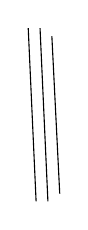
\begin{tikzpicture}[x=1mm,y=1mm]\draw (0,0)--(-1,22);\draw (1.5,0)--(0.5,22);\draw (3,1)--(2,21);\end{tikzpicture}}

\scanpage{64}
% archive foliation: 63
\unsure{soient|sont} des isomorphismes, avec le complément que $\uline{H^{\unsure{0|i}}(X,M)\text{ est un}}$ $\mathbf{Q}$-\uline{module de type fini}.
\figure{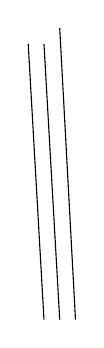
\begin{tikzpicture}[x=1mm,y=1mm]\draw (0,0)--(-2,35);\draw (2,0)--(0,35);\draw (4,0)--(2,37);\end{tikzpicture}}

\deleted{Ceci doit être valable en particulier dans les deux cas \unsure{typiques} suivants
\[
\begin{array}{ll}
\text{a)}&X\text{ de type fini sur }\mathbf{Z}\\
\text{b)}&X\text{ de type fini sur un corps alg. clos.}
\end{array}
\]}

En particulier, pour un corps alg. clos $k$, on aura
\[
H^i(k,M)=0\quad\text{pour }i>0,\qquad \forall\text{ motif }M.
\]

\uline{NB} Si $X$ est de type fini (ou projectif lisse) sur un corps alg. clos $K$, \unsure{on n'a plus de} telles relations précises, comme on voit par calcul explicite (utilisant les conjectures de Tate) pour $K$ clôture algébrique d'un corps fini ----

Le th de Tate peut se reformuler et se préciser en énonçant :
\[
A^i(X)\otimes_{\mathbf{Z}}\mathbf{Q}\inserted{\nearrow\ \unsure{\text{pas}|\text{pr}}\ \mathbf{Q}_\ell}\simeq \Gamma_k(R^i f_*(\mathbf{Q}_X(\unsure{i|0})))
\]

\scanpage{65}
% archive foliation: 64
$X$ étant projectif et lisse sur $k$ alg. clos, morphisme structural $f:X\longrightarrow\mathrm{Spec}\,k$.

\uline{Une autre façon est celle-ci}
\[
\boxed{A^i(X)\deleted{\otimes\mathbf{Q}_\ell}\simeq\mathrm{Im}\left[H^{2i}(X,\mathbf{Q}(i))\longrightarrow H^{2i}(X,\mathbf{Q}_\ell(i))\right]}
\]

\uline{NB.} Si $k$ est la clôture algébrique de $\mathbf{F}_p$, \unsure{on devrait} pour $X$ projectif lisse sur $k$
\[
H^{\unsure{i|2i}}(X,\mathbf{Q}(j))\inserted{\nearrow\ \uline{\text{pas}}\ \mathbf{Q}_\ell(i)!}=
\begin{cases}
0&\text{si }i\ne 2j,2j+1\\
A^i(X)\otimes_{\mathbf{Z}}\mathbf{Q}&\text{si }i=2j\quad\text{(canonique)}\\
A^{\unsure{i|j}}(X)\otimes_{\mathbf{Z}}\mathbf{Q}&\text{si }i=2j+1\quad\text{(\uline{pas} canonique)}
\end{cases}
\]
De plus, pour $i\ne 2j$, l'image de $H^i(X,\mathbf{Q}(j))$ dans $H^i(X,\mathbf{Q}_\ell(j))$ est nulle.

C'est un \uline{fait général} : si $k$ alg. clos, alors (si $X$ projectif lisse sur $k$) l'image de
\[
H^{\unsure{j|i}}(X,\mathbf{Q}(\unsure{i|j}))\longrightarrow H^{\unsure{j|i}}(X,\mathbf{Q}_\ell(i))
\]
est \uline{nulle} pour $j\ne 2i$ (question de poids) ; pour $j=2i$ ce sont les cycles algébriques \inserted{à coeffs} rationnels.

\scanpage{67}
% archive foliation: 66
Notons le \uline{th. de dualité absolue} :

Soient $M$ et $M^*$ deux \inserted{(complexes de)} motifs sur $X$ (de type fini sur $\mathbf{Z}$), qui sont ``duals'' pour le \deleted{$\unsure{[|\xi}$} complexe de motifs dualisants \deleted{$\unsure{]|\xi}$} canonique --- [NB Si $X$ est régulier \inserted{partout} de dim $n$, alors c'est la dualité à valeurs dans \deleted{$\unsure{\mathbf{Q}(n)[2n]|\mathbf{Q}(n)[n]}$}\inserted{$\mathbf{Q}(n)[2n+1]$}\margin{shift}\deleted{\unsure{shift}}]

alors $\mathbf{R}\Gamma_X(M)$ et $\unsure{R|\mathbf{R}}_!\Gamma_X(M^*)$ \inserted{``\unsure{support pr} sur $\mathrm{Spec}\,\mathbf{Z}$''} sont duals. Ici [Comme les coefficients sont \unsure{ess.} $\mathbf{Q}$\unsure{\}}, donc il n'y a pas de $\mathrm{Tor}$]

ceci revient aussi à la formule (cas régulier)
\[
\boxed{\begin{array}{lll}
H^i(X,M)&\text{dual de}&\mathrm{Ext}_!^{2n+1-i}(X;M,\mathbf{Q}(n))\\
H^i_!(X,M)&\text{dual de}&\mathrm{Ext}^{2n+1-i}(X;M,\mathbf{Q}(n))
\end{array}}
\]
Si $X$ propre sur $\mathrm{Spec}\,\mathbf{Z}$, inutile de mettre des $!$.

Moyennant le thm de dualité \uline{relative} pour motifs, cet énoncé revient au

\scanpage{71}
% archive foliation: 70
$X$ \unsure{projective|projectif} lisse \inserted{géo. connexe} sur $k$ corps fini à $q$ éléments.
Par passage à la limite sur les \deleted{\unsure{quotients}} \inserted{coefficients} finis, on trouve
\diagram{\begin{tikzcd}[column sep=small]
0\arrow[r]&H^{i-1}(\overline{X},\mathbf{Q}_\ell(j))_\pi\arrow[r]&H^i(X\deleted{^{\unsure{\circ}}},\mathbf{Q}_\ell(j))\arrow[r]&H^i(\overline{X},\mathbf{Q}_\ell(j))^\pi_{\deleted{\unsure{\pi}}}\arrow[r]&0
\end{tikzcd}}
d'où le résultat
\[
\text{si }i\ne2j,2j+1,\qquad H^i(X,\mathbf{Q}_\ell(j))=0
\]
si $i=2j$
\diagram{\begin{tikzcd}
H^{2j}(X,\mathbf{Q}_\ell(j))={}&H^{2j}(\overline{X},\mathbf{Q}_\ell(j))^\pi\arrow[d,phantom,"\wr" description,"\text{Conj. de Tate}"]\\
&A^j(X/k)\otimes_{\unsure{\mathbf{Z}|\mathbf{Q}}}\mathbf{Q}_\ell
\end{tikzcd}}
si $i=2j+1$
\diagram{\begin{tikzcd}
H^{2j+1}(X,\mathbf{Q}_\ell(j))={}&H^{2j\deleted{\unsure{+1}}}(\overline{X},\mathbf{Q}_\ell(j))_\pi\arrow[d,phantom,"\wr" description,"\substack{\text{Tate + action}\\\text{semi-simple}}"]\\
&A^j(X/k)\otimes_{\unsure{\mathbf{Z}|\mathbf{Q}}}\mathbf{Q}_\ell
\end{tikzcd}}

Soit maintenant $k_n$ l'extension de degré $n$ de $k$ dans $\overline{k}$, et étudions
\[
\varinjlim_n H^i(X_{k_n},\mathbf{Q}_\ell(j))
\]
on trouve $0$ pour $i\ne2j,2j+1$ ; pour $i=2j$, on trouve
\[
H^{2j}(\overline{X},\mathbf{Q}_\ell(j))^{\unsure{\mathfrak{g}|0}}=A^j(\overline{X})\otimes_{\unsure{\mathbf{Z}|\mathbf{Q}}}\mathbf{Q}_\ell,
\]
enfin pour $i=2j+1$, on trouve également $A^j(\overline{X})\otimes_{\mathbf{Z}}\mathbf{Q}_\ell$.
Donc on \unsure{trouve} \inserted{\unsure{du pt de vue motifs}}
\[
\begin{array}{rcl}
\varinjlim H^i(X_{k_n},\mathbf{Q}(j))&=&\begin{cases}
0&\text{si }i\ne2j,2j+1\\
A^j(\overline{X})\otimes_{\unsure{\mathbf{Z}|\mathbf{Q}}}\mathbf{Q}&\text{si }i=2j\deleted{,2j+1}\\
\deleted{\unsure{A^j(\overline{X})}}\ \mathrm{id}&\text{si }i=2j+1,
\end{cases}\\
\Vert&&\text{mais pas \uuline{canoniquement} en }\unsure{k}\ !\\
H^i(\overline{X},\mathbf{Q}(j))&&\inserted{\unsure{fonctoriellement}}
\end{array}
\]
\margin{\uline{N.B.} \unsure{Remplacer} $k$ par $k_n$ revient à multiplier l'isom obtenu par \unsure{$n$} ---}

\scanpage{72}
% archive foliation: 71
% Typescript is upside down in the supplied whole-page orientation.
\deleted{
Ceci donne une démonstration plus sympatique et élémentaire de 11.9.6. Quant à 11.9.3. (ii), il varésulter d'un

\uline{Lemme} (ou corollaire à la proposition précédente). Sous les hypothèses de la proposition, ne supposons plus néc que $A'$ soit projectif sur $A$, mais seulement ceci: pour tout quotient intègre $B=A/\underline{p}$ de $A$, posant $B'=B\otimes_A A'$, il existe un $h\ B-(0)$ tel que $B_h$ soit \deleted{projectif} \inserted{libre} sur $A_h$.
Alors la conclusion de la proposition reste encore valable.

Soit en effet $\phi$ une section de $F'$ dont les images par les $u'$ sont nulles, prouvons $\phi=0$, i.e. $\mathrm{supp}\,\phi=\varnothing$. Dans le cas contraire, il existerait un point maximal $x'$ dans $\mathrm{supp}\,\phi$, correspondant à l'idéal premier $\underline{p}'$ de $A'$. Soit \deleted{$\underline{p}=\unsure{\underline{p}'\cap A'|\underline{p}'\cap A}$} \inserted{$x$} son image dans $X$, défini par l'idéal $\underline{p}$ trace de $\underline{p}'$ sur $A$, alors en vertu de l'hypothèse appliquée à $A/\underline{p}$, on voit que, quitte à remplacer $X$ par un voisinage ouvert affine de $x$, on peut supposer que $\unsure{A'|B'}/\underline{p}B'$ est \deleted{projectif} \inserted{libre} sur $A/\underline{p}$. Notons que nous pouvions choisir $x'$ de façon que $x$ soit également maximal dans $g(\mathrm{supp}\,\phi)$ (commencer par choisir $x$ maximal dans $g(\mathrm{supp}\,\phi)$, puis $x'$ maixmal dans $g^{-1}(x)$), ce qui signifie que localisant en $\underline{p}$, le support de $\phi_{\underline{p}}$ est contenu dans $\mathrm{Spec}(A'_{\underline{p}}/\underline{p}A'_{\underline{p}})$, donc $\phi_{\underline{p}}$ est annulé par une puissance de $\underline{p}\,A'_{\underline{p}}$, ou encore que l'on peut trouver $h\ A-\underline{p}$ tel que
}

\scanpage{73}
% archive foliation: 72
$S$ \inserted{lisse} de \deleted{\unsure{t}} type fini sur $\mathbf{F}_p$.

$M$ motif \unsure{ct tordu|et tordu} de poids $\rho$
\margin{? ---}
\[
H^*(S,M_\ell)\overset{\deleted{\unsure{?}}}{\Longleftarrow}H^p(\mathbf{F}_p,R^qf_*(M_\ell))
\]
\diagram{\begin{tikzcd}[column sep=small]
0\arrow[r]&\underbrace{H^{i-1}(\overline{S},\overline{M}_\ell)_\pi}_{\substack{\text{poids entre}\\\rho+i-1\text{ et }\rho+\mathrm{Inf}(\unsure{2i-2|2i},2n)}}\arrow[r]&H^i(S,M_\ell)\arrow[r]&\underbrace{H^i(\overline{S},\overline{M}_\ell)^\pi}_{\substack{\text{poids entre}\\\rho+i\text{ et }\rho+\mathrm{Inf}(2i,2n)}}\arrow[r,dash]&0
\end{tikzcd}}
Donc $H^i(S,M_\ell)=0$ \deleted{\unsure{si on a}} sauf si on a
\[
\rho+i-1\le0\le\rho+2i-2\quad\uline{\text{ou}}\quad\rho+i\le0\le\rho+2i
\]
i.e.
\[
2-2i\le\rho\le\deleted{\unsure{2}}1-i\quad\uline{\text{ou}}\quad-2i\le\rho\le-i
\]
i.e.
\[
\begin{array}{ll}
-2i\le\rho\le-i+1&(\deleted{\unsure{\{}}\text{ si }i\ge2)\\
-2\le\rho\le1&(\text{si }i=1)\\
\rho=0&(\text{si }i=0)
\end{array}
\]
\deleted{Pour $i=1$, on \unsure{trouve}}
\[
\unsure{\rho}
\]
\figure{\begin{tikzpicture}[x=8mm,y=8mm]
\draw (0,0)--(4,0);\draw (0,-.13)--(0,.13);\draw (.6,-.02)--(.6,.3);\draw (3.5,-.12)--(3.5,.3);\draw (4,0)--(4,.15);
\node[below] at (0,-.25) {$-2i$};\node[above] at (.6,.35) {$-2i+2$};\node[below] at (3.5,-.2) {$-i$};\node[above] at (4,.35) {$-i+1$};
\end{tikzpicture}}
\deleted{\figure{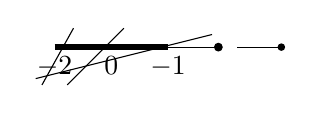
\begin{tikzpicture}[x=8mm,y=8mm]
\draw[line width=2pt] (0,0)--(1.8,0);\draw (1.8,0)--(2.6,0);\draw (2.9,0)--(3.6,0);\fill (2.6,0) circle(.07);\fill (3.6,0) circle(.06);
\node[below] at (0,0) {$-2$};\node[below] at (.9,0) {$\unsure{0}$};\node[below] at (1.8,0) {$-1$};
\draw (-.2,-.6)--(.3,.3);\draw (-.3,-.5)--(2.5,.2);\draw (.2,-.6)--(1.1,.3);
\end{tikzpicture}}}
\figure{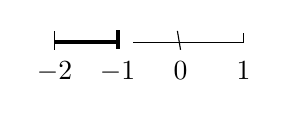
\begin{tikzpicture}[x=8mm,y=8mm]
\draw[line width=1.4pt] (0,0)--(1,0);\draw (1.25,0)--(3,0);\draw (0,-.12)--(0,.18);\draw[line width=1.4pt] (1,-.1)--(1,.2);\draw (2,-.12)--(1.95,.18);\draw (3,0)--(3,.15);
\node[below] at (0,-.15) {$-2$};\node[below] at (1,-.15) {$-1$};\node[below] at (2,-.15) {$0$};\node[below] at (3,-.15) {$1$};
\end{tikzpicture}}

\scanpage{74}
% archive foliation: 73
\uline{\mspage{16}}
Relations avec les pts \deleted{\unsure{d}} rationnels \inserted{et la cohomologie} des Variétés abéliennes sur un \deleted{corps de type fini} \inserted{schéma de type fini} ...

Soit $A_K$ VA sur corps $K$ de \uline{type fini} pour commencer. Alors $K$ est le corps de fonctions d'un schéma $S$ irréductible et régulier, de type fini sur $\mathbf{Z}$, \deleted{et} \inserted{tel que} $A_K$ provient d'un schéma abélien sur $S$.

De plus, on a
\[
A_K(K)=A(S)
\]
et on sait que c'est un \uline{groupe de type fini} par Mordell--Weil--Néron--Lang.

Soit $f:A\longrightarrow S$ la projection, et considérons le motif
\[
R^1\unsure{f^*|f_*}(\mathbf{Q}_{A^*}(\unsure{1|0}))\simeq\deleted{\unsure{H^1(A)|H_\ell(A)}}\inserted{T_{\mathrm{motif}}(A)}
\]
\inserted{[où $A^*$ est le dual de $A$]}
qui est un motif ct tordu sur $S$ \deleted{de} pur de poids $1$, qui redonne $A_K$ à isogénie près \deleted{sur $\unsure{K|\overline{K}}$} (sur $K$ ?) comme l'indiquent les conjectures de Tate.

\scanpage{75}
% archive foliation: 74
On s'attend donc à pouvoir écrire $A(S)\otimes_{\mathbf{Z}}\mathbf{Q}$ en termes de ce motif $M$.
\unsure{Or|Et} en effet, des raisons heuristiques convaincantes \deleted{\unsure{que}} nous suggèrent
\[
A(S)\otimes_{\mathbf{Z}}\mathbf{Q}\simeq H^1(S,T_{\mathrm{mot}}(A))
\]
[NB. On doit avoir $H^0(S,T_{\mathrm{mot}}(A))=0$, à cause de \deleted{Mordell--Weil} considérations de poids ---].
\deleted{Une autre façon de} \inserted{Considérons \unsure{donc} le processus} \unsure{(aux $\ell$ inversibles à $X$)}
\diagram{\begin{tikzcd}[column sep=small]
\unsure{0|\varnothing}\arrow[r]&{}_{\ell^\nu}A\arrow[r,dash]&A\arrow[r,dash]&A\arrow[r,dash]&0
\end{tikzcd}}
d'où
\diagram{\begin{tikzcd}[column sep=small]
0\arrow[r]&H^0(S,A)_{\ell^\nu}\arrow[r,dash]&H^1(S,{}_{\ell^\nu}A)\arrow[r]&{}_{\ell^\nu}H^1(S,A)\arrow[r,dash]&0
\end{tikzcd}}
et par passage à la limite et $\otimes_{\mathbf{Z}_\ell}\mathbf{Q}_\ell$
\diagram{\begin{tikzcd}[column sep=small]
0\arrow[r]&\underbrace{H^0(S,A)}_{\substack{\text{de type fini}\\\text{sur }\mathbf{Z}}}\otimes_{\mathbf{Z}}\mathbf{Q}_\ell\arrow[r]&H^1(S,T_\ell^{\deleted{\unsure{\mathbf{Q}}}}(A))_{\mathbf{Q}_\ell}\arrow[r]\arrow[d,phantom,"\wr" description]&T_{\unsure{\cdot|\ell}}^{\deleted{\unsure{\mathbf{Q}}}}(H^1(S,A))_{\mathbf{Q}_\ell}\arrow[r]&0\\
&&H^1(S,T_{\mathrm{mot}}(A))\otimes_{\mathbf{Q}}\mathbf{Q}_\ell&&
\end{tikzcd}}
et le résultat escompté ici équivaut visiblement à celui-ci :
\[
\boxed{\begin{array}{l}
H^1(S,A)(\ell)\quad\uuline{\text{fini}}\quad\text{si }\ell\text{ ``premier à }S\text{''}\\
\hfill(S\text{ de type fini sur }\mathrm{Spec}\,\mathbf{Z})
\end{array}}
\]
p.ex. si $S=\mathrm{Spec}\,\mathbf{F}_q$, alors il est vrai par Lang !

\scanpage{76}
% archive foliation: 75
Si $S$ est de type fini sur $\mathbf{F}_p$, on aura (travaillant avec des \uline{faisceaux étales}) si $f:S\unsure{-|\longrightarrow}\mathrm{Spec}\,\mathbf{F}_p$
\diagram{\begin{tikzcd}[column sep=small]
0\arrow[r]&H^1(\mathbf{F}_p,R^0f_*A)\arrow[r]&H^1(S,A)\arrow[r]&H^0(\mathbf{F}_p,R^1f_*(A))\arrow[r]\arrow[d,phantom,"\Vert" description]&0\ \deleted{\unsure{H^2(\mathbf{F}_p,R)}}\\
&&&H^1(\overline{S},\overline{A})^\pi&
\end{tikzcd}}
Or on a, tjrs par ``Kummer''
\diagram{\begin{tikzcd}[column sep=small]
0\arrow[r]&\overset{\inserted{M\otimes\mathbf{Q}_\ell/\mathbf{Z}_\ell}}{H^0(\overline{S},\overline{A})\otimes\mathbf{Q}_\ell/\mathbf{Z}_\ell}\arrow[r,dash]&H^1(\overline{S},{}_{\ell^\infty}\overline{A})\arrow[r]&H^1(\overline{S},\overline{A})(\ell)\arrow[r]&0
\end{tikzcd}}
d'où le fait que $H^1(\overline{S},\overline{A})(\ell)$ est de poids $1-1=0$ \inserted{si p.ex. $S$ est projectif lisse sur $\mathbf{F}_p$} --- à priori rien ne s'oppose à ce qu'il y ait un gros module d'invariants. D'autre part, on a
\diagram{\begin{tikzcd}[column sep=small]
0\arrow[r,dash]&\underbrace{A^{\mathrm{fix}}}_{\substack{\unsure{\text{partie fixe}}\\\text{de la V.A. }A\text{ sur }S}}\arrow[r]&R^0f_*(A)\arrow[r]&\underbrace{M}_{\substack{\pi\text{-module,}\\\text{de type fini sur }\mathbf{Z}}}\arrow[r,dash]&0
\end{tikzcd}}
d'où
\diagram{\begin{tikzcd}[column sep=small]
H^1(\mathbf{F}_p,A^{\mathrm{fix}})\arrow[r,dash]\arrow[d,phantom,"\Vert" description]&H^1(\mathbf{F}_p,R^0f_*(\unsure{M|A}))\arrow[r]&H^1(\mathbf{F}_p,M)\arrow[r]\arrow[d,phantom,"\Vert" description]&0\\
\substack{0\\\text{par Lang}}&&(\underline{M}\otimes\mathbf{Q}/\mathbf{Z})^\pi&
\end{tikzcd}}

\scanpage{77}
% archive foliation: 76
Si $S$ de type fini sur $\mathbf{F}_p$, on obtient le diagramme suivant
\margin{(b)}
\diagram{\begin{tikzcd}[column sep=small,row sep=large]
&M^\pi\otimes\mathbf{Q}_\ell/\mathbf{Z}_\ell\arrow[d,phantom,"\wr" description]&&&\\
0\arrow[r]&H^0(S,A)\otimes\mathbf{Q}_\ell/\mathbf{Z}_\ell\arrow[r,dash]\arrow[d]&H^1(S,{}_{\ell^\infty}A)\arrow[r,dash]\arrow[d]&H^1(S,A)(\ell)\arrow[r,dash]\arrow[d]&0\\
0\arrow[r,dash]&(H^0(\overline{S},\overline{A})\otimes\mathbf{Q}_\ell/\mathbf{Z}_\ell)^\pi\arrow[r,dash]\arrow[d,phantom,"\wr" description]&H^1(\overline{S},{}_{\ell^\infty}\overline{A})^\pi\arrow[r,dash]&H^1(\overline{S},\overline{A})(\ell)^\pi\arrow[r,dash]&0\\
&(M\otimes\mathbf{Q}_\ell/\mathbf{Z}_\ell)^\pi&&&
\end{tikzcd}}
\figure{\begin{tikzpicture}[x=1mm,y=1mm]\draw (0,0)--(.2,3);\draw (0,2)--(2,2);\draw (.2,3)--(2,3.2);\end{tikzpicture}}

[où $M=H^0(\overline{S},\overline{A})/H^0(\overline{\mathbf{F}}_p,\overline{A}^{\mathrm{fix}})$, $\pi$ est le groupe de Galois de $\overline{\mathbf{F}}_p$ sur $\mathbf{F}_p$]

Les déterminations $H^0(S,A)\simeq M^\pi$ et $H^0(\overline{S},\overline{A})\otimes\mathbf{Q}_\ell/\mathbf{Z}_\ell\simeq M\otimes\mathbf{Q}_\ell/\mathbf{Z}_\ell$ sont \unsure{standart|standard} ; on sait que la première flèche verticale est un isomorphisme mod groupes finis. D'autre part, on trouve (suite spectrale de Leray de $f:S\longrightarrow\mathrm{Spec}\,\mathbf{F}_p$ pour la \uline{top. étale})
\diagram{\begin{tikzcd}[column sep=small]
0\arrow[r,dash]&H^1(\mathbf{F}_p,R^0f_*(A))\arrow[r,dash]\arrow[d,phantom,"\wr" description]&H^1(S,A)\arrow[r,dash]&H^0(\mathbf{F}_p,R^1f_*(A))\arrow[r,dash]\arrow[d,phantom,"\Vert" description]&0\\
&\text{groupe fini}&&H^1(\overline{S},\overline{A})^\pi_{\deleted{\unsure{\pi}}}&
\end{tikzcd}}
\inserted{$\curvearrowright$ comme on voit utilisant}
\diagram{\begin{tikzcd}[column sep=small]
0\arrow[r,dash]&\unsure{\overline{A}|\widetilde{A}}^{\mathrm{fix}}\arrow[r,dash]&R^0f_*(A)\arrow[r,dash]&M\arrow[r,dash]&0
\end{tikzcd}}
, et le

\scanpage{78}
% archive foliation: 77
\figure{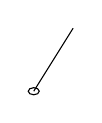
\begin{tikzpicture}[x=1mm,y=1mm]\draw (0,0) ellipse(.7mm and .45mm);\draw (0,0)--(5,8);\end{tikzpicture}}
$H^2(S,A)\deleted{\unsure{\otimes\mathbf{Q}_\ell}}$ (dont le $T_\ell$ est $H^2(S,T_\ell(A))$) n'est pas néc nul, \deleted{\unsure{si}} \inserted{comme on voit} si $S$ est une courbe lisse projective géom. connexe sur $\mathbf{F}_p$ et $A=J\times S$, où $J$ est la jacobienne de $S$.
On a en tous cas
\[
\begin{aligned}
H^2(S,T_\ell(A))&\simeq H^1(\overline{S},T_\ell(\overline{A}))_\pi\\
&=\deleted{T_\ell J(\overline{\mathbf{F}}_p)\otimes}\inserted{[T_\ell(\unsure{\check{J}|\overline{J}})\otimes T_\ell(\overline{J})]_\pi}\\
&\simeq\mathrm{End}(J)\otimes_{\unsure{\mathbf{Z}|\mathbf{Q}}}\mathbf{Q}_\ell\quad\deleted{\unsure{par}}\ (\simeq(\unsure{\text{bihom}|\text{classes}}\text{ de corr. }\inserted{\text{divisorielles}}\text{ sur }C\,C)\otimes_{\mathbf{Z}}\mathbf{Q}_\ell
\end{aligned}
\]
qui est non nul .....

\scanpage{79}
% archive foliation: 78
fait $H^1(\mathbf{F}_p,A^{\mathrm{fix}})=0$ (Lang) et $H^1(\mathbf{F}_p,M)=\text{fini}$ [\unsure{triv.|trivial} ; Attention qu'il s'agit de la coh. \uline{étale}, i.e. de la coh. \uline{galoisienne} de $\widehat{\mathbf{Z}}$ !], donc la dernière flèche verticale du diagramme (\unsure{D|b}) est aussi bijective :
\[
H^1(S,A)(\ell)\xrightarrow{\sim}H^1(\overline{S},\overline{A})^\pi(\ell)
\]
\margin{\uline{surj. à noyau fini} ...}
Donc la \uline{conjecture} précédente signifie aussi
\[
\boxed{H^1(\overline{S},\overline{A})(\ell)^\pi=\text{groupe fini}}
\]

\deleted{Il y a une façon de le prouver,}
C'est \inserted{aussi} $\pm$ équiv. (via des jacobiennes) à ceci : $X\unsure{-|\longrightarrow}S$ morphisme propre [lisse de dim relative $1$], $S$ régulier de type fini sur $\mathbf{Z}$. Prouver que
\[
H^2(S,\mathbf{G}_m)\longrightarrow H^2(X,\mathbf{G}_m)
\]
est surjectif mod groupes finis ??
\figure{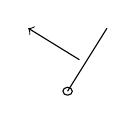
\begin{tikzpicture}[x=1mm,y=1mm]\draw (0,0) ellipse(.6mm and .5mm);\draw (0,0)--(5,8);\draw[->] (1.5,4)--(-5,8);\end{tikzpicture}}

\margin{\uline{NB} On devrait avoir $H^{\unsure{2|i}}(S,A)(\ell)$ fini aussi pour $\uuline{i\ge3}$, $S$ de type fini sur $\mathbf{Z}$, $\ell$ premier avec \unsure{car.} visiblement \unsure{on} (\inserted{\uline{NB}} si $i\ge2$, $T_\ell(H^i(S,A)(\ell))\simeq H^i(S,T_\ell(A))$)}
\margin{\unsure{donc les seuls} \illegible{1} \unsure{qui restent} sont $H^0$ et $H^2$ pour $A$, et \deleted{$\unsure{H^0}$}, $H^1$, $H^2$ pour $T_\ell(A)$}

\scanpage{80}
% archive foliation: 79
\unsure{Noter|Notons} que
\[
H^1(S,\deleted{\unsure{A}}T_\ell(A))\simeq H^1(\overline{S},T_\ell(\overline{A}))^\pi
\]
Donc notre conjecture signifie essentiellement
\[
\mathrm{rang}_{\mathbf{Q}_\ell}(H^1(\overline{S},T_\ell(\overline{A}))^\pi\simeq\mathrm{rang}_{\mathbf{Z}}A(K)
\]
et sous cette forme est essentiellement équivalente à la \uline{conjecture de} \deleted{\unsure{Swy}} \uline{Birch--Swinnerton Dyer}.

\scanpage{82}
% archive foliation: 81
$C$ courbe lisse \inserted{propre} sur $\mathbf{F}_{\unsure{q|p}}$

$A$ schéma abélien sur $C$.

Des conjectures de Weil, résulte que
\[
H^i(C,A)=0\qquad\text{si }i\ge2
\]
et sans doute, utilisant Tate, on doit avoir
\[
H^1(C,A)=0
\]
Soit $x$ un pt fermé de $C$, $U=C-\{x\}$, alors on a
\diagram{\begin{tikzcd}[column sep=small]
\deleted{\unsure{H^0(C,A)}}\arrow[r,dash]&\deleted{\unsure{H^1_x(C,A)}}\arrow[r]\arrow[d,dashed]&H^1(C,A)\arrow[r]\arrow[d,phantom,"\Vert" description]&H^1(U,A)\arrow[r]&H^2_x(C,A)\arrow[r]&H^2(C,A)\arrow[d,phantom,"\Vert" description]\\
&0&0&&&0
\end{tikzcd}}
d'où
\[
H^1(U,A)\simeq H^2_x(C,A)
\]
Or par Tate,
\[
H^2_x(C,A)\deleted{\unsure{(\ell)}}\quad H^1(K_x,A)\deleted{\unsure{(\ell)}}\quad\uline{\text{dual}}\text{ de }H^0(K_x,A^*)\deleted{\unsure{(\ell)}}
\]
\deleted{\unsure{Ce n'est en général pas un groupe de}}
C'est \uuline{donc essentiellement un $p$-groupe}, modulo groupe fini !

OK.

Peut se généraliser au cas où on prend $X$ régulier dont on enlève un diviseur \uline{régulier} ----

\scanpage{84}
% archive foliation: 83
\uline{Calculs} pour $T_\ell(\mathbf G_m)\inserted{{}=\mathbf Q_\ell(1)}$ et $\mathbf G_m$.

$X$ de type fini sur $\mathbf Z$

\[
H^0(X,\mathbf Q_\ell(1))\deleted{\unsure{\mathbf G_m}}=0
\]
\figure{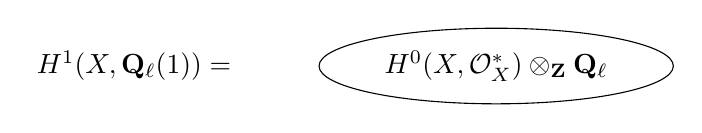
\begin{tikzpicture}
\node at (0,0) {$H^1(X,\mathbf Q_\ell(1))=$};
\node at (4.6,0) {$H^0(X,\mathcal O_X^*)\otimes_{\mathbf Z}\mathbf Q_\ell$};
\draw (4.6,0) ellipse (2.25 and .48);
\end{tikzpicture}}
\figure{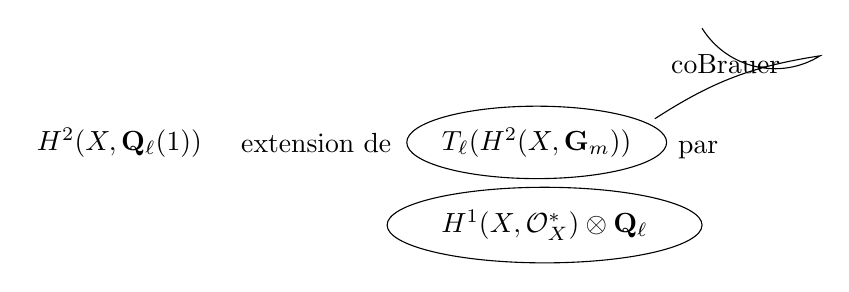
\begin{tikzpicture}
\node at (0,0) {$H^2(X,\mathbf Q_\ell(1))$};
\node at (2.5,0) {extension de};
\node at (5.3,0) {$T_\ell(H^2(X,\mathbf G_m))$};
\draw (5.3,0) ellipse (1.65 and .46);
\node at (7.35,-.1) {par};
\node at (5.4,-1.05) {$H^1(X,\mathcal O_X^*)\otimes\mathbf Q_\ell$};
\draw (5.4,-1.05) ellipse (2 and .48);
\node at (7.7,1) {\uline{coBrauer}};
\draw (6.8,.3) to[bend left=12] (8.9,1.1) to[bend left=45] (7.4,1.45);
\end{tikzpicture}}
\[
H^3(X,\mathbf Q_\ell(1))\simeq T_\ell(H^3(X,\mathbf G_m))\quad\text{est ce qu'il peut}
\]
\hfill [p.ex. $\mathbf Z_\ell$ si $X$ \deleted{\unsure{modèle}} \unsure{cour.} d'un
corps de fonctions d'une variable sur $\mathbf F_p$]

\[
\begin{array}{c}
H^i(X,\mathbf Q_\ell(1))=0\\
\Vert\\
T_\ell(H^i(X,\mathbf G_m))
\end{array}
\qquad\text{si }i\ge4\qquad ??
\]

On conjecture (C. Artin) que $H^2(X,\mathbf G_m)=$ groupe
fini si $X$ propre sur $\mathbf Z$. \deleted{Alors si}\inserted{Vrai}
si $X$ courbe projective lisse sur $\mathbf F_p$, mais
faux quand on lui enlève des pts --- le
rang du $H^{\unsure{2|3}}$ augmente d'autant.

$H^{\unsure{3|2}}(X,\mathbf Q_\ell(1))$ : quelle est sa taille [il décroît en
passant à un ouvert de $X$]

\scanpage{86}
\mspage{17}
% archive foliation: 85
\uline{Formes positives}

Le thème étant géométrique, nous nous plaçons
sur un corps alg. clos $k$. Nous ne
considérons que des motifs $\frac12$ \uline{simples}
sur $k$, \inserted{purs} de poids $\rho$. Soit $M$ un tel
motif, considérons les formes
\[
M\times M\longrightarrow\mathbf Q(-\rho)
\]
i.e. les éléments de
\[
\Gamma_k\bigl(\mathcal Hom(M\otimes M,\mathbf Q(-\rho))\bigr)=\Phi(M)
\]
où le \deleted{$\Gamma_k$ \unsure{est}} $\mathcal Hom$ est bien de poids $0$.
Elles forment un vectoriel de \deleted{poids $0$}\inserted{dim finie}
sur $\mathbf Q$. On considère l'\inserted{\unsure{sous-}}espace des
formes \uline{symétriques} si
$\rho$ pair, \uline{alternées} si $\rho$ impair. Cet
espace sera noté $\Phi^s(M)$. Noter les
hom canoniques
\[
\Phi^s(M)\otimes\Phi^s(N)\longrightarrow\Phi^s(M\otimes N)
\]

\scanpage{87}
% archive foliation: 86
par produit tensoriel des formes
[N.B. le produit tensoriel de deux formes
\deleted{symétriques, ou de} de même type de symétrie
est symétrique --- de deux types opposés
de symétrie est antisymétrique]. Bien
entendu, ils ne sont pas en général
bijectifs (mais du moins injectifs).

On a aussi
\[
\Phi^s(M'\times M'')\simeq\Phi^s(M')\times\Phi^s(M'')\times B(M',M'')
\]
où $B(M',M'')=\operatorname{Hom}(M'\otimes M'',\mathbf Q(\rho))$.

Ceci posé, on \deleted{\unsure{aura pour $d$}}\inserted{a dans}
$\Phi^s(M)$ un cône \inserted{convexe} fermé $\Phi^+(M)$.
\figure{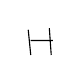
\begin{tikzpicture}[scale=.4]
\draw (0,0)--(-.08,.8) (0,.46)--(.7,.46) (.65,0)--(.59,.85);
\end{tikzpicture}}
On a les propriétés suivantes :

(i) $\Phi^+(M)$ a un intérieur non vide.

(ii) Un élément de $\Phi^+(M)$ est dans l'int. de $\Phi^+(M)$ ssi il est non dég.

\margin{formes $\in\Phi^+(M)$ sont dites pseudo-amples, celles
dans l'intérieur sont dites \uline{amples}}

(iii) Pour $M\longrightarrow N$, $\Phi^+(N)$ s'envoie dans $\Phi^{\unsure{s|+}}(M)$.

(iv) \deleted{\unsure{(iii)} \unsure{Pour}} Si $M\longrightarrow N$ injectif,
\deleted{$\Phi^+(\unsure{N|M})$} l'intérieur
de $\Phi^+(N)$ s'envoie dans l'intérieur
de $\Phi^+(M)$ (forme ample $\longrightarrow$ forme ample)

\scanpage{88}
% archive foliation: 87
\deleted{\unsure{(v)|(iv)}}\deleted{\unsure{(iv)|(iii)}}
i.e. la forme induite sur $M$ \inserted{par une forme ample}
est non dégénérée,
donc $N=M\oplus M^\perp$, et la forme sur
$N$ est la somme des formes induites sur
$M$, $M^\perp$.

(v) La somme directe de deux formes
\deleted{positives \unsure{ou}} pseudo-amples (amples) est
itou.

(vi) Le produit tensoriel de deux formes
amples est ample.

(vii) Si $\rho=0$, de sorte que essentiellement $M$
est défini par un vectoriel de dim
finie sur $\mathbf Q$, alors les formes amples
sont les formes \uline{définies positives}.
\deleted{\unsure{Énoncé} analogue pour $M(\rho)$, $M$ un vectoriel
de dim finie sur $\mathbf Q$; utilisant
l'isom canon}

(viii) Cas de $\mathbf Q(\rho)$ : on a $\Phi^s(\mathbf Q(\rho))\simeq\mathbf Q$,)
et on veut que les formes amples
correspondent aux nbs \inserted{\uline{strict}} \uline{positifs}.

\scanpage{89}
% archive foliation: 88
De (vi) et (viii) résulte que pour tt
motif $M$ et entier $n$, l'isomorphisme
\[
\Phi^s(M)\simeq\Phi^s(M(n))
\]
est compatible avec les cônes amples.

De (iv) et \unsure{(vi)|(vii)} résulte que si $\rho=0$, une
forme ample sur $M$ induit une
forme \uline{définie positive}
\[
\Gamma_k M\times\Gamma_k M\longrightarrow\Gamma_k\mathbf Q(0)=\mathbf Q
\]

Si on décompose $M$ (de poids $\rho$) en
composantes isotypiques $M_\alpha$, il vient
\[
\Phi^s(M)\simeq\unsure{\prod|\bigoplus}_\alpha\Phi^s(M_\alpha)
\]
donc pour étudier les formes positives, il
suffit de les étudier en principe sur
des morceaux isotypiques, qui sont
d'ailleurs \unsure{sous|de} la forme
\[
I\otimes_A\unsure{V|W}
\]
où $I$ est un motif simple, $A$ son
anneau des endomorphismes, qui est
un corps, et $\unsure{V|W}$ un \uline{vectoriel} sur $A$

\scanpage{90}
\figure{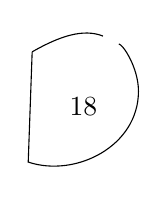
\begin{tikzpicture}[x=1mm,y=1mm]
\node at (0,0) {\mspage{18}};
\draw (-6.5,7)--(-7,-7) .. controls (-1,-9) and (7,-5) .. (7,2) .. controls (7,5) and (5,8) .. (4.5,8);
\draw (-6.5,7) .. controls (-3,9) and (0,10) .. (2.5,9);
\end{tikzpicture}}
% archive foliation: 89
\uuline{Dictionnaire}\qquad Fonctions $L$ --- \unsure{Cohomologie} à
\hfill action galoisienne.

Soit $k$ un \deleted{corps} anneau

\deleted{$\unsure{\mathcal A|\mathbf N}$ la catégorie}
\deleted{$\operatorname{Mod}(\mathbf Z)$ la catégorie}
$C$ la catégorie des modules de longueur
finie sur $k[t]=$ \deleted{vectoriels}\inserted{modules} $V$ \inserted{proj.}
de \deleted{dim}\inserted{rang} finie sur
$k$ munis d'un endomorphisme $f=$
$k[\unsure{\mathbf N|\mathbf Z}]$-modules, de \deleted{\unsure{rang}}\inserted{projectifs} finie sur $\unsure{\forall k|k}$.

Cette catégorie donne lieu à un faux-anneau,
noté $R^\bullet(\unsure{\mathbf N|\mathbf Z};k)$, qui est aussi, \inserted{si $k$ est un corps,}
le \deleted{\unsure{faux-anneau}} \inserted{groupe}
libre engendré par les classes des $k[\unsure{\mathbf N|\mathbf Z}]$-
modules simples, \inserted{finis sur $k$} or on connaît les $k[t]$-modules
simples, ce sont les polynômes \inserted{unitaires} irréductibles
$P\in k[t]$, en associant à $P$ le module
$k[t]/Pk[t]$. À tout tel $P$, \inserted{est} associé \unsure{à}
un $(V,f)$, dont le polynôme car. est
précisément $P$,
\margin{$k$ un corps ou non}
\[
P(t)=\det(t\,\mathrm{id}-f)
\]
[vrai pour $\forall P$, irréd. ou non !]. Il nous sera
plus commode de remplacer $P(t)$ par
\[
Q(t)=t^dP\left(\frac1t\right)=\det(1-tf)
\]
qui est un polynôme quelconque à coeff. cst égal $1$.

\scanpage{91}
% archive foliation: 90
Ainsi, on obtient via le pol. car. modifié un
hom
\[
(V,f)\longmapsto\frac1{\det(\mathrm{id}_V-ft)}=L(V,f)
\]
\[
R(\unsure{\mathbf N|\mathbf Z};k)\longrightarrow 1+k[[t]]^+
\]
\inserted{\unsure{Composé|Conjugué} avec l'\deleted{\unsure{isomorphisme|homomorphisme}}\inserted{aut° ``additif''}
$\varphi(t)\longmapsto\dfrac1{\varphi(t)}$ dans $1+k[[t]]^+$}
qui est un hom de $\lambda$-anneaux,
\margin{\figure{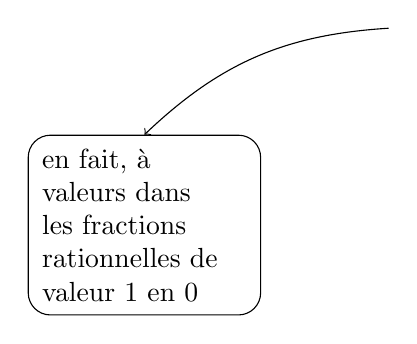
\begin{tikzpicture}[x=1cm,y=1cm]
\node[draw,rounded corners=8pt,align=left,text width=2.6cm,inner sep=5pt] (note) at (0,0) {en fait, à valeurs dans les \uline{fractions rationnelles} de valeur $1$ en $0$};
\draw[->] (3.1,2.5) to[bend right=20] (note.north);
\end{tikzpicture}}}

Lorsque $k$ est un corps, l'hom
précédent est injectif. En effet, si
\deleted{$k$ est \unsure{alg. clos},} la connaissance de la
série formelle permet de reconstituer \inserted{la fonction rationnelle}
[$k[t]$
étant factoriel] l'élément
$\displaystyle\sum_{\substack{P\ \unsure{pol.|irr.}\\\mathrm{unitaires}}}c_P(V_P,f_P)$
\deleted{dont} par
\[
L=\prod_Q Q^{c_P}
\]
[$Q$ et $P$ associés de
la façon précisée plus haut].

Notons qu'on a un homomorphisme
naturel \deleted{\unsure{$k$ séparé alg.}}
\[
1+k[[t]]^+\longrightarrow k[[t]]
\]
\[
\varphi(t)\longmapsto\frac{\varphi'(t)}{\varphi(t)}\deleted{\unsure{t}}
\]
qui correspond à
\[
\Lambda(V,f)(t)=\frac{L(V,f)'(t)}{L(V,f)(t)}
=[\log L(V,f)]'=\frac1t\sum_1^\infty(\operatorname{Tr}f^n)t^n.
\]
\deleted{En car. $0$, on peut}
Si $k$ de car. $0$, \inserted{i.e. $k\supset\mathbf Q$} on peut inverser cet
homomorphisme par $\exp\left(\int_0^{\unsure{t}}\Lambda(V,f)(t)\right)$.
Donc \inserted{si $k$ est \margin{un corps de car. $0$,}}
$\Lambda:R(\mathbf N,k)\longrightarrow k[[t]]$ est aussi injectif \deleted{($k$ corps}

\scanpage{92}
% archive foliation: 91
Si $k$ n'est pas de car. $0$, on ne peut en
général aller en sens inverse, et
$R(\mathbf N,k)\xrightarrow{\Lambda}k[[t]]$ n'est \deleted{en général} pas injectif,
[$k$ corps de car. $>0$]

\figure{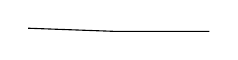
\begin{tikzpicture}\draw (0,0)--(1.1,-.04)--(2.3,-.04);\end{tikzpicture}}

On voit \deleted{que} par la formule de
Lefschetz-Weil-Grothendieck que la connaissance
de la fonction $L$ de $\unsure{(X,F)|X}$ algébrique
sur $\mathbf F_p$, \inserted{à coeff dans $F$,} \uline{équivaut} à celle de l'élément
\[
\uline{\chi}(F)=\sum(-1)^i\,\mathrm{cl}\,H^i_!(\bar X,\bar F)
\quad\text{de }R(\mathbf N,\mathbf Q_\ell)
\]
[car essentiellement cette fonction $L$ est l'image
de $\uline{\chi}(F)$ dans $1+\mathbf Q_\ell[[t]]^+$]. Lorsque
on admet les conjectures de Weil, et $F$
\inserted{est un motif,}
$\uline{\chi}(F)$ se décompose suivant les poids en
\[
\sum(-1)^i\,\deleted{\unsure{\mathrm{cl}}}\uline{h}^i_!(F),
\qquad\uline{h}^i(F)\in R(\mathbf N,\mathbf Q_\ell),
\]
et la \deleted{\unsure{connaiss.}} connaissance de $L(X,F)(t)$
\uline{équivaut} à celle des $\uline{h}^i(F)$ : les $\uline{h}^i(F)$
correspondent à la décomposition de $L(X,F)$

\scanpage{93}
% archive foliation: 92
\deleted{\unsure{somme|sommes}} en groupant suivant les valeurs absolues
des zéros et pôles\ldots. Lorsque $X$ est
complet et lisse, \inserted{et $F$ \unsure{localement tordu|constant tordu}, de poids $\rho$,}
on a $\uline{h}^i(F)=H^{i-\rho}_!(\bar X,\bar F)$
comme $\mathbf N$-modules, donc on a la
connaissance de $L(X,F)$ équivaut à celle des
$H^{\unsure{i-\rho|i}}(\bar X,\bar F)$ et l'opération du Frobénius dedans.

\deleted{
\diagram{\begin{tikzcd}
X \arrow[r,dash] \arrow[d] & X_{(\unsure{\eta})}\arrow[d,dash]\\
Y \arrow[r,dash] & K
\end{tikzcd}}
$K=$ corps des fonctions de $Y$

Soit $f:X\mathbin{-}Y$ morphisme
[non propre] avec $X,Y$ algé-
briques de type fini sur $\mathbf F_p$.
Considérons les ouverts
denses $U$ de $Y$, et
les $L(f^{-1}(U),F)$. Pour $U$ variable, les
fonctions rationnelles
}

Considérons, d'autre part \inserted{[pour $X$ de dim $n$]}
les ouverts \deleted{denses} $U$ de $X$, \inserted{tels que $X-U$ de dim $<n$,} et les
$L(U,F\vert U)$, qui ne diffèrent \deleted{que} (pour $F$ pur
de poids $\rho$) que par des fonctions rationnelles
de poids $\le2n-2+\rho$. Donc, à priori la
\margin{les poids ici sont pour la bonne filtration \deleted{\unsure{voir}} N°12}
connaissance de l'invariant birationnel
$L(X,F)$ mod. fonct. rat. de poids $\le2n-2+\rho$,

\scanpage{94}
% archive foliation: 93
\uline{équivaut} à celle de
$\mathrm{cl}\,H^{2n}_!(X,F)-\mathrm{cl}\,H^{2n-1}_!(X,F)$
mod. les $=$ choses. On peut supposer $X$
[affine et] lisse sur $\mathbf F_p$, \inserted{(\deleted{\unsure{pure}}\inserted{\unsure{purement}} de dim $n$)} alors $H^{2n}_!(X,F)$
est dual de
\[
H^0(X,\mathcal Hom(F,\mathbf Q_\ell(n)))=H^0(X,\check F)(n),
\]
\inserted{donc} purement de poids $2n$. D'autre part, $H^{2n-1}_!(X,F)$
est dual de $H^1(X,\mathcal Hom(F,\mathbf Q_\ell(n)))$, et admet
une pièce de poids $2n-1$ \uline{et} des poids $2n-2$.
\margin{\uline{peut se raffiner}, \uline{en regardant une}
\uline{autre filtration} \uline{que par les poids},
\uline{savoir \unsure{le niveau|la dimension}}}

\deleted{Une analyse}
Si $F=\mathbf Q_\ell(0)$, \deleted{alors} donc
\deleted{le cas} si on s'occupe des fonctions $\zeta$
habituelles, la connaissance ``birationnelle
grossière'' de $\zeta$ est essentiellement équivalente à :
celle de $\pi_0(\bar X)$ comme Frob-ensemble,
et celle de l'Albanèse de $X$ sur $\mathbf F_p$\ldots
\margin{Modulo conjectures de Tate}

Une analyse plus serrée \deleted{\unsure{de ces faits}} (plus
fine que par les seuls \uline{poids}, mais en
utilisant aussi les niveaux) permet de
récupérer plus par la connaissance de
$\zeta(X\deleted{,F})$ \inserted{(disons, en prenant $F=\mathbf Q_\ell$)} modulo les
$\zeta(Y\deleted{,\unsure{F}})$ ($\dim Y<n$)
\deleted{poids $\unsure{\le\rho}$}

\scanpage{95}
% archive foliation: 94
savoir les ``invariants birationnels fondamentaux''
\inserted{relativement à $\mathbf F_p$,}
\deleted{de} envisagés dans les notes sur les \uline{Motifs}.

Il semblerait opportun d'étudier \deleted{\unsure{si}}
\inserted{le cas des coefficients $F$ généraux et de voir si,}
pour un morphisme $f:X\longrightarrow Y$
disons lisse \deleted{projectif}\inserted{propre}, \inserted{$F$ \unsure{lct|ct} tordu sur $X$,} la connaissance de
\deleted{$\unsure{H|\zeta}$}
$L(X,F)$ modulo $L(f^{-1}(Y'),F)$,
pour $Y'$ propre dans $Y$, permet de récupérer
les invariants birationnels fondamentaux
de $(X_K,\unsure{F\vert_{X_K}|F\vert_K})/K$
[$K$ corps des fonctions de
$Y$]. \uline{Dans quelle mesure faut-il}
\uline{faire les hypothèses $f$ lisse propre}, et $F$
\uline{ct tordu} pour obtenir des énoncés
de cette nature ??
\figure{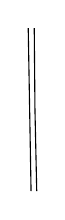
\begin{tikzpicture}[scale=.45]
\draw (0,0)--(-.04,2.3)--(-.08,4.6) (.16,0)--(.11,2.3)--(.09,4.6);
\end{tikzpicture}}

\scanpage{96}
% archive foliation: 95
Poids et niveaux des
espaces de cohomologie
$\ell$-adiques (base var.
quelconque)
